\chapter{Wykonanie projektu}
\label{cha:course}

\section{Projekt płytki}
\subsection{Schemat}
Projekt płytki, naturalnie rozpoczęto od wykonania schematu ideowego. W tym celu przyjęto następujące założenia:
\begin{itemize}
    \item Układ, musi być zasilany zewnętrznie (5v oraz 3.3V)
    \item Wykorzystany zostanie konwerter UART-USB
    \item Układ, będzie można wyłączyć tranzystorem, sterującym przetwornicami
    \item Wykorzystany zostanie zewnętrzny generator
\end{itemize}
Według standardu mikroBUS\texttrademark, płytka zasilana jest przez układ w który jest wpięta. Często jest to zasilanie procesora, na którym tworzone jest oprogramowanie. Ponieważ w opisywanym projekcie, wykorzystany został procesor, oraz trzy sensory (w tym jeden pracujący z napięciem 5V), zdecydowano się na zasilanie zewnętrzne. Miało ono zminimalizować prawdopodobieństwo nieprawidłowej pracy układu. Jednocześnie, czujnik MQ2 pobierając setki mA prądu, mógłby uszkodzić przetwornicę układu w który została wpięta płytka. Najprostszym rozwiązaniem, było wyprowadzenie portu USB i zasilanie z niego układu. Zwrócono uwagę na fakt, że USB w komputerach, nie ma stabilnego napięcia 5V, a często wręcz 4.7-4.8V. Jest to zachowanie zdefiniowane w standardzie USB 2.0 \cite{usb_specification} w rozdziale 7. Z tego powodu , należało wykorzystać regulator napięcia. \newline Wybór tego i wszystkich kolejnych komponentów, podyktowany był w dużej mierze dostępnością na rynku. Kolejnym kryterium, były parametry układu, opisywane w dostarczanych przez producentów dokumentacjach. Jako układ do zasilania sensora MQ2, wykorzystano przetwornicę typu BOOST - MCP1642 o wyjściowym napięciu właśnie 5V. Pozwoliła ona na stabilne zasilenie czujnika. Jej ważną cechą, jest maksymalny prąd na wyjściu, o wartości 800mA. Wysoki prąd jest tutaj niezbędny, ponieważ zasilanie wspomnianego czujnika wymaga nawet 200mA prądu stałego. Do zasilania reszty elementów, wykorzystano regulator LDO  MIC5365 o wyjściowym napięciu 3.3V. Gwarantowany prąd wyjściowy regulatora to 150mA, co jest wartością wystarczającą do zasilenia reszty elementów z zapasem. Całość, z założenia włączana miała być tranzystorem NMOS 2N7002. Bramka tego tranzystora, połączona jest z pinem RESET standardu mikroBUS\texttrademark, pozwalając użytkownikowi wyłączyć układ. W przypadku tego elementu, pojawiły się dwa błędy, wymagające przerobienia gotowej płytki. Problem, szerzej opisano w podrozdziale \ref{sub:mistakes}. \newline
Schemat oraz layout, wykonane zostały w programie KiCad. Opensourcowym oprogramowaniu dla różnych systemów operacyjnych. Program ten, umożliwia podział schematu na bloki, co wykorzystano przenosząc sekcję zasilania do osobnego schematu. Na schemacie \ref{img:power_sch} przedstawiono całą, wspomnianą sekcję. Zasilanie, doprowadzone jest z USB do obu przetwornic. Gdy procesor jest zasilony, a więc działa przetwornica 3.3V, włączona zostaje czerwona dioda LED. Widoczny na schemacie rezystor R10, nie jest uwzględniony w layoucie i został dołożony ręcznie do płytki. Więcej na ten temat, opowiada podrozdział \ref{sub:mistakes}.
\newline Na schemacie, widoczna jest również znacząca ilość kondensatorów. Zostały one dodane do schematu, jako wskazane przez producenta jako konieczne dla poprawnego działania układów. Bardzo istotny jest również rezystor R7, gwarantujący ustalony stan niski po wyłączeniu tranzystora.
\begin{figure}[H]
    \centering
    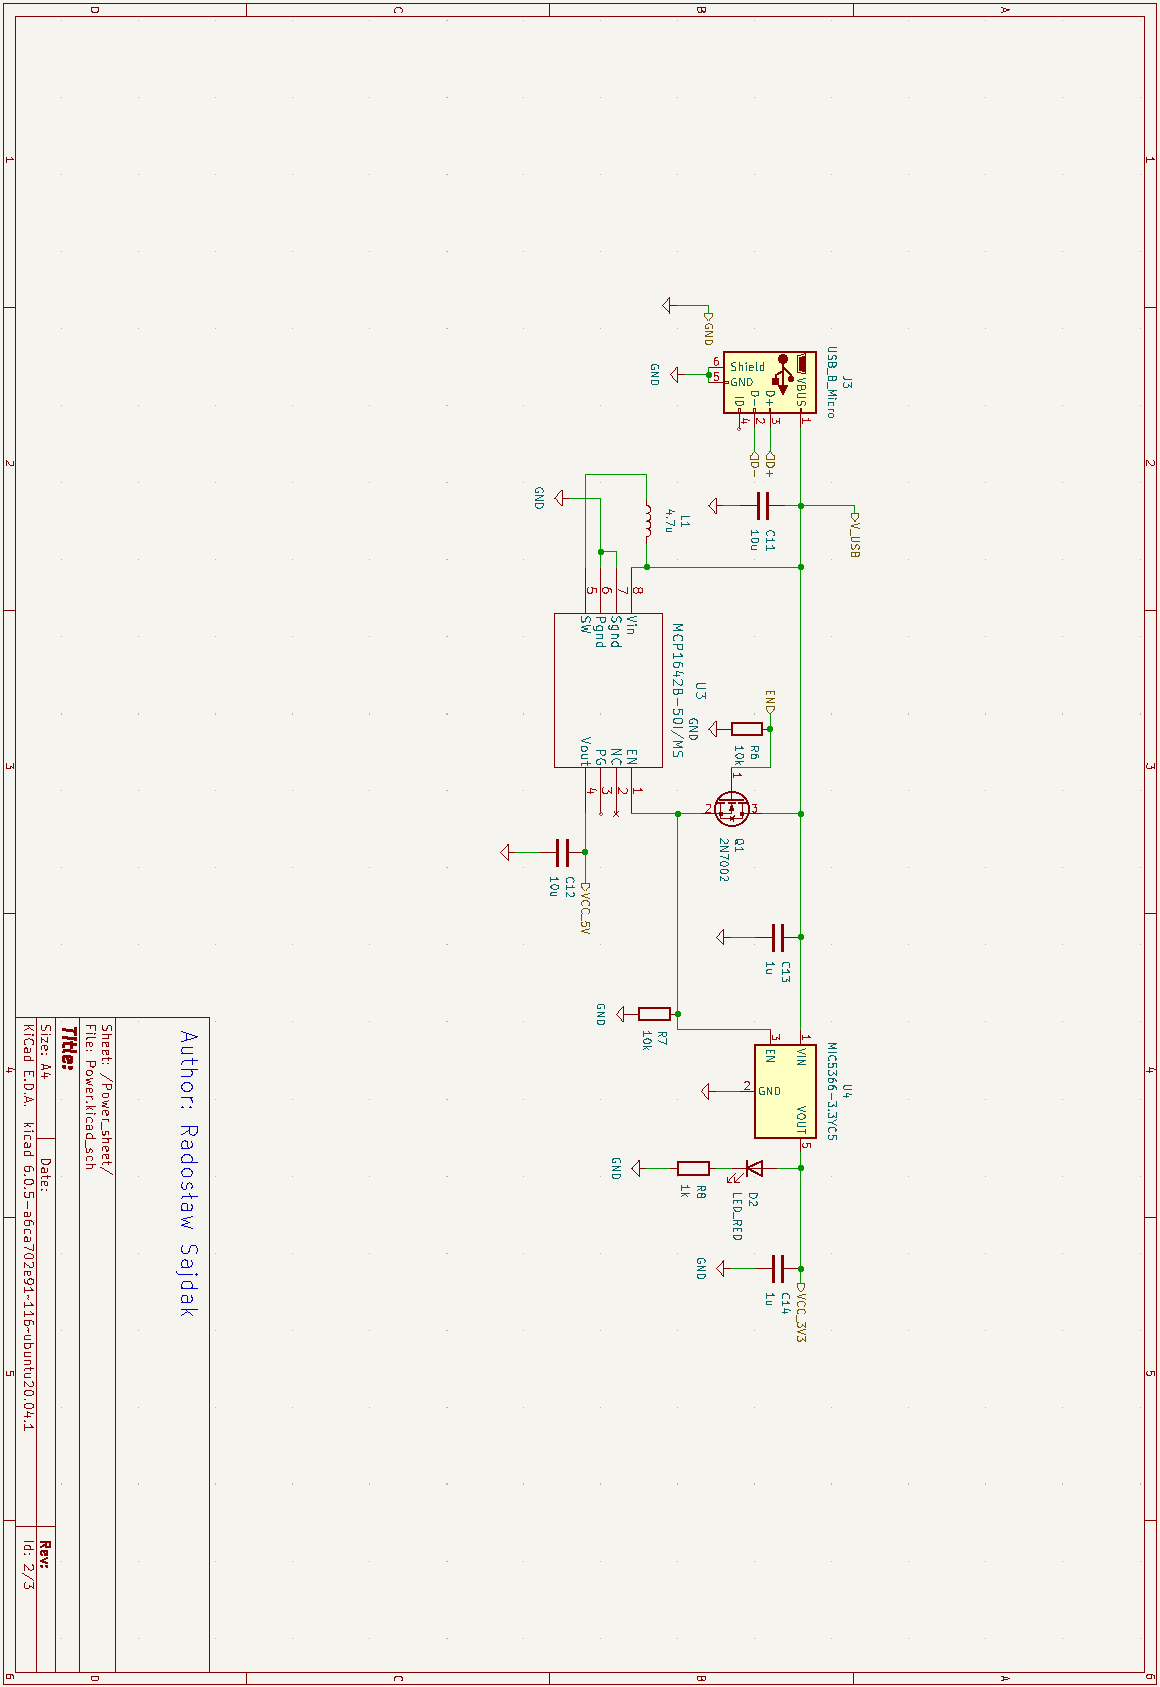
\includegraphics[width=\textwidth, height=\textheight, keepaspectratio]{Graphics/power_sch.png}
    \caption{Schemat części zasilającej moduł}
    \label{img:power_sch}
\end{figure}
Kolejnym blokiem, jest schemat \ref{img:sensors_sch}, zawierający w sobie wszystkie czujniki. Podobnie jak wcześniej, producenci w swoich dokumentacjach zalecają stosowanie kondensatorów, jak najbliżej zasilania układu, dla zapewnienia jego prawidłowego działania. W przypadku sensora działającego z użyciem SPI - BMP280 - zastosowano rezystor pull-down na linii MISO. Dzięki temu, gdy linia nie jest używana, zagwarantowany jest stan niski. Podobnie w przypadku linii NSS. Zastosowanie rezystora podciągającego do zasilania, pozwala zagwarantować, że układ nie będzie aktywny gdy nie jest to pożądane.\newline
Wartym uwagi jest układ czujnika analogowego MQ2. Ze względu na zastosowany procesor, mierzone przetwornikiem napięcie, musi mieścić się w przedziale 0-3.6V. Ponieważ wybrany czujnik działa w zakresie 0-5V, konieczne jest zastosowanie dzielnika napięcia. W tym przypadku, układ rezytorów oraz czujnika, staje się źródłem prądu, który mógłby uszkodzić procesor. Z tego powodu, zastosowano wzmacniacz operacyjny w konfiguracji nieodwracającego wtórnika napięciowego. Wzmacniacz operacyjny, mający bardzo małą rezystancję wyjściową, stanowi w przybliżeniu źródło napięcia równe co do wartości spadkowi napięcia na R11.
\newline
\newline
Ostatnim, a zarazem najistotniejszym, jest schemat \ref{img:main_sch}. Po jego lewej stronie, zaznaczono fragment odpowiadający za konwersję UART-USB. Wykorzystany układ konwertera to CP2102. Układ ten, pozwala obserwować logi mikroprocesora przy użyciu tego samego przewodu, którym zasilamy płytkę. W trakcie tworzenia schematu, rozważano również tylko wyprowadzenie testpointów, pozwalających na podejrzenie logów zewnętrznym konwerterem. Ponieważ jednak planowany jest również inny projekt, wykorzystujący wiele takich konwerterów, zdecydowano się na jego użycie w celach przede wszystkim edukacyjnych i testowych. Głównym zagadnieniem z nim z związanym, było użycie pary różnicowej, wymaganej dla prawidłowegodziałania USB.
\newline
Po prawej stronie schematu \ref{img:main_sch}, widoczny jest blok mikroprocesora STM32F103C8. Zastosowano tutaj zewnętrzny generator o taktowaniu 8MHz, zastępując wewnętrzny zegar mikroprocesora. Istotnym zaganieniem, wymaganym przez mikroprocesor według dokumentacji, jest montaż osobnych kondensatorów o wartości 100n przy każdym z pinów zasilania, możliwie jak najbliżej układu. Dla zapewnienia prawidłowego działania magistrali I$^2$C, dodano rezystory podciągające linie do zasilania. Wszystkie piny posiadają też testpointy, mające ułatwić tworzenie oprogramowania dzięki szybkiemu wykryciu błędów w transmisji, a więc np. w zlutowaniu układu. Dodatkowo, na pinie 8, wyprowadzono LED. Zgodnie z przyjętymi przez zespół założeniami, wskazuje on gotowość układu do pracy, a więc przejście wszystkich kroków inicjalizacyjnych.
\newline
Wartym zaznaczenia jest tutaj fakt nie wyprowadzenia pinów SWDIO oraz SWCLK. Ponieważ są to piny wymagane tylko na etapie tworzenia oprogramowania, podjęto decyzję o ich niewykorzystaniu. Ważną w tym wypadku kwestią, był również brak miejsca na ścieżki, pozwalające na taki zabieg. Niemniej jednak, osoba składająca PCB, bez większych problemów była w stanie wlutować przewody programatora bezpośrednio do pinów mikroprocesora.
\begin{figure}[H]
    \centering
    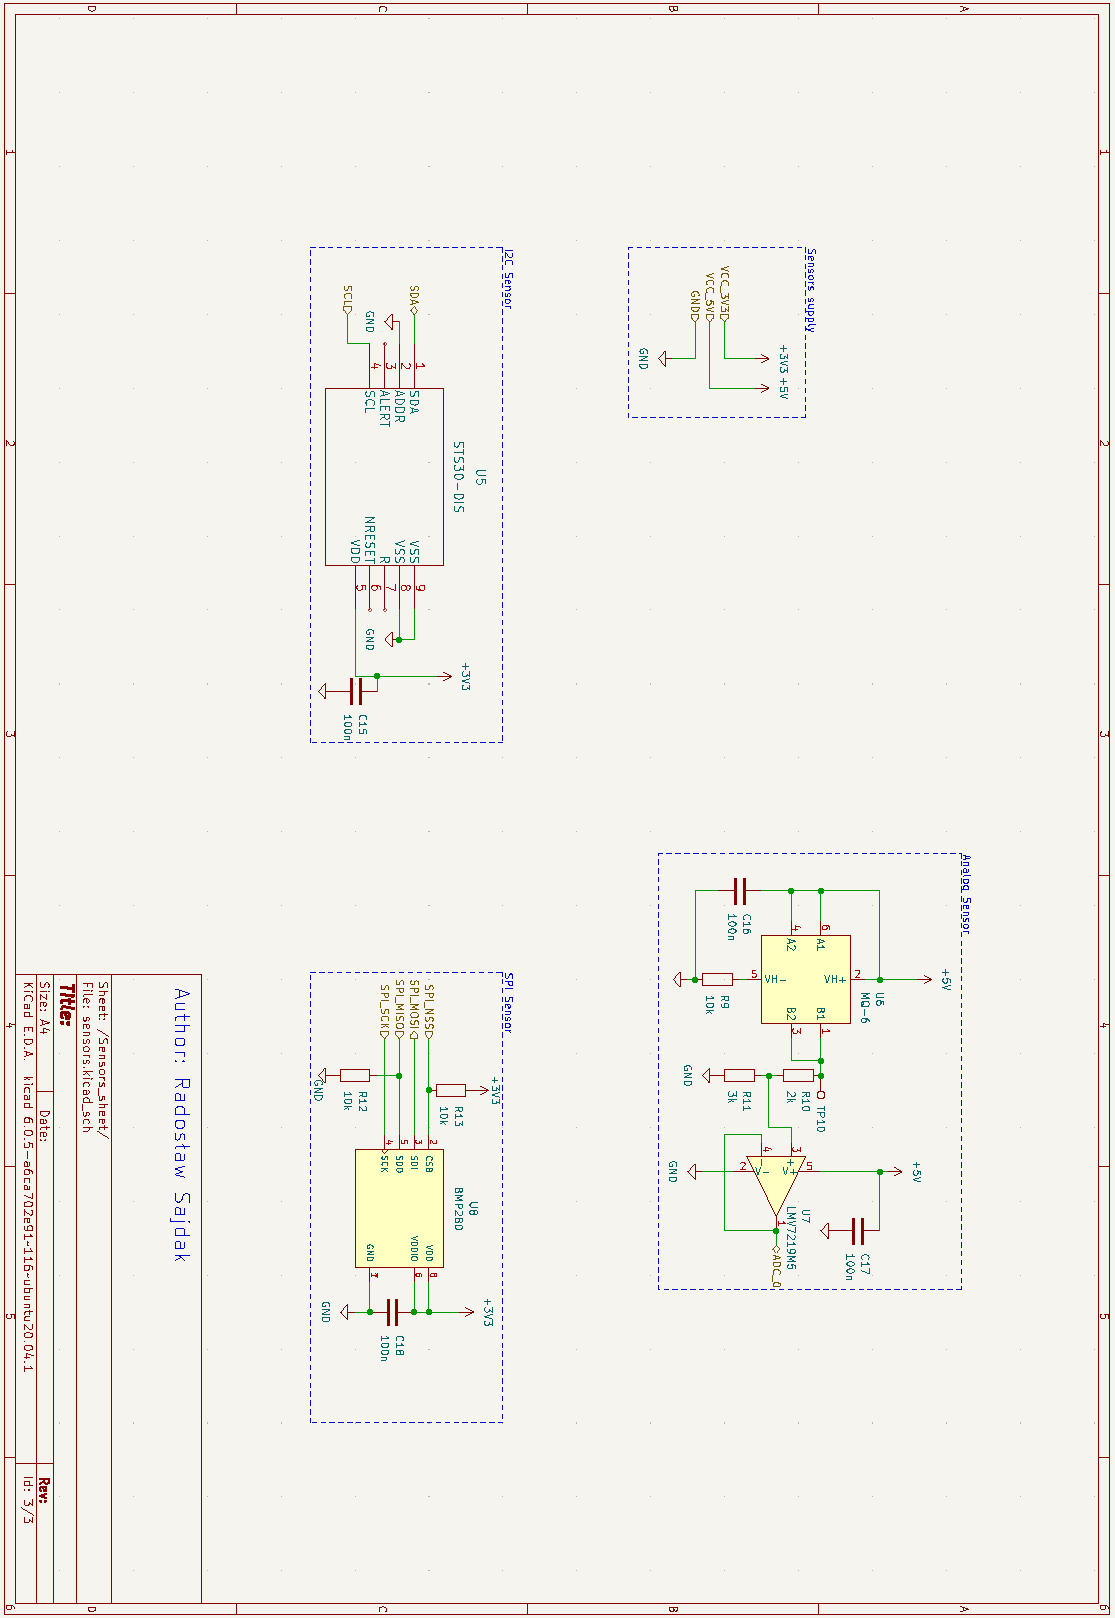
\includegraphics[width=\textwidth, height=\textheight, keepaspectratio]{Graphics/sensors_sch.png}
    \caption{Schemat połączeń czujników}
    \label{img:sensors_sch}
\end{figure}
\begin{figure}[H]
    \centering
    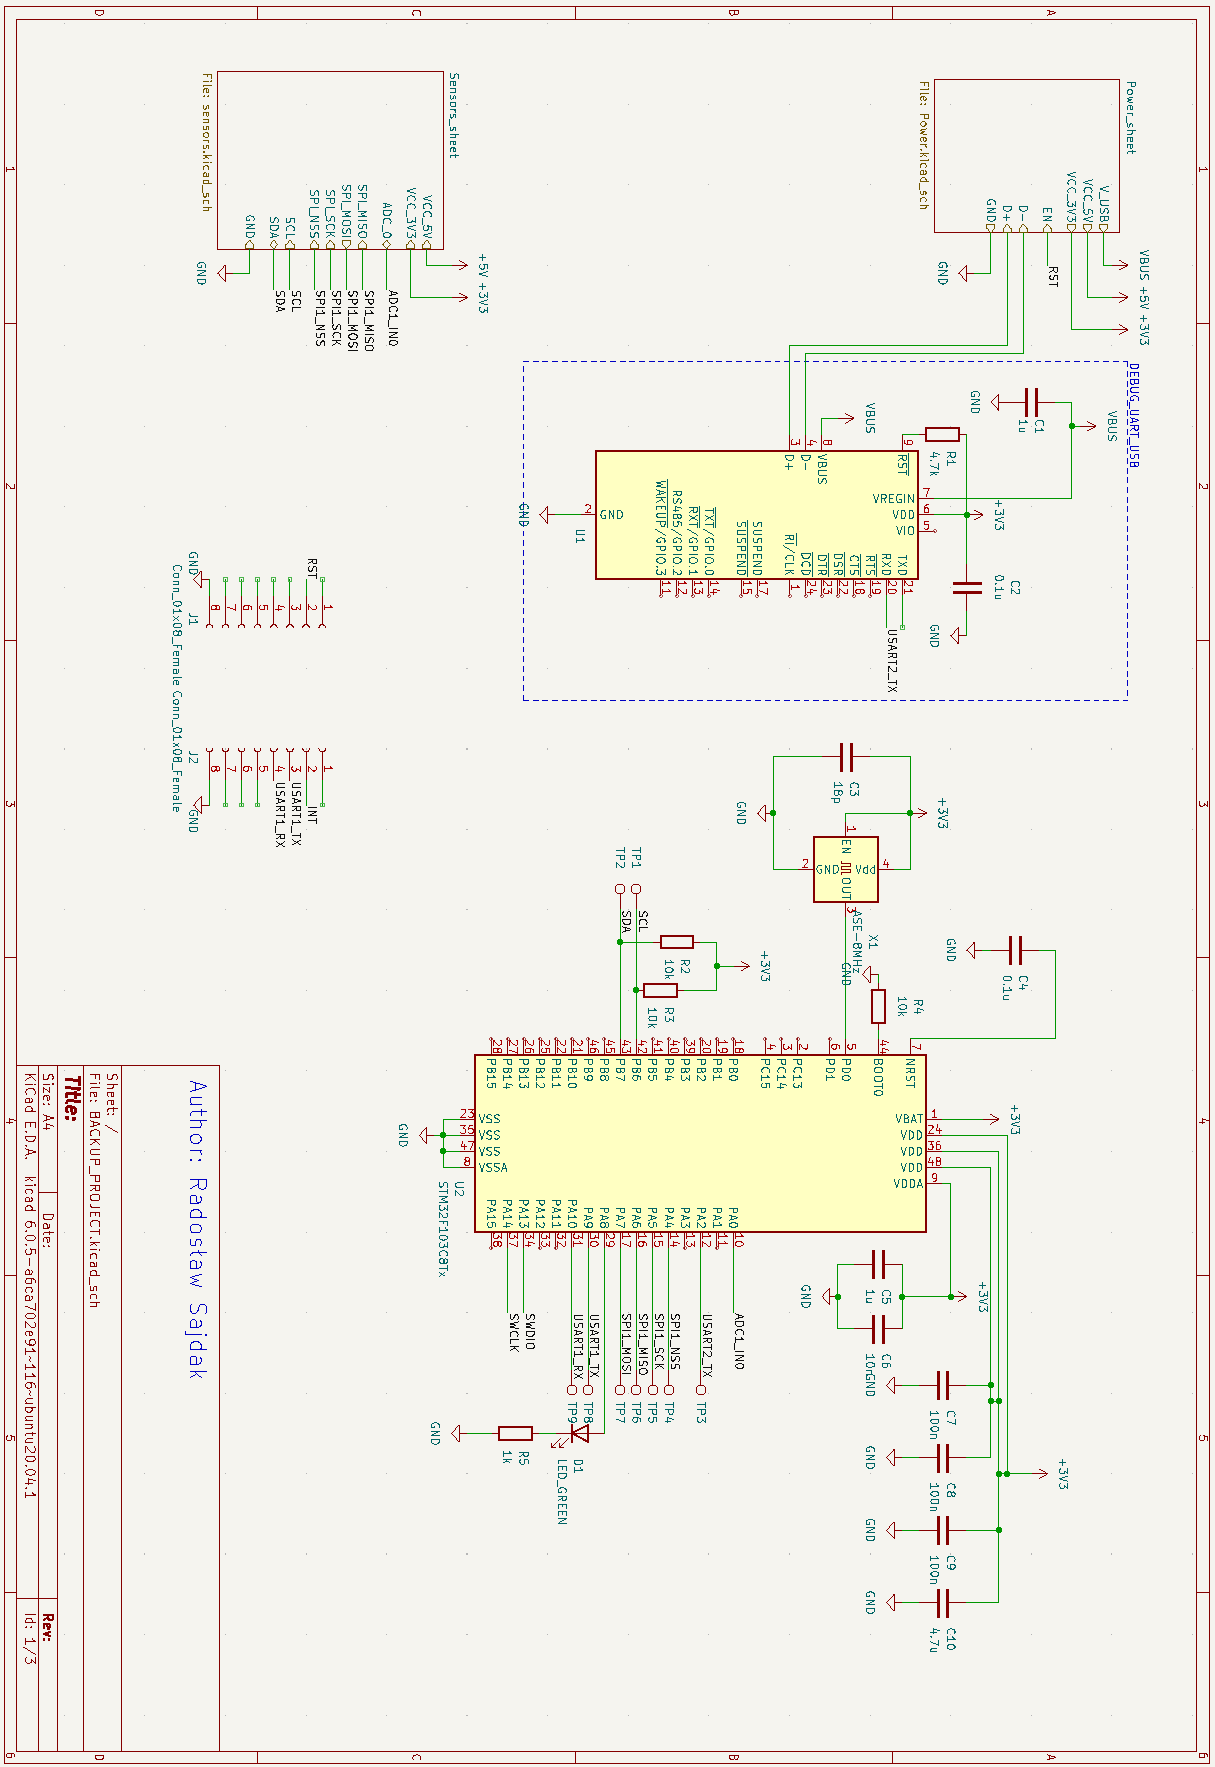
\includegraphics[width=\textwidth, height=\textheight, keepaspectratio]{Graphics/main_sch.png}
    \caption{Schemat połączeń konwertera UART-USB oraz mikroprocesora}
    \label{img:main_sch}
\end{figure}
\subsection{Layout}
\textbf{Pokazać warstwy elektryczne. Zdjęcia wydrukowanych płytek. Jakie problemy się pojawiły (1 raz z Kicadem, więc np. okazało się, że domyślnie ścieżki ma całkiem szerokie. Podobnie viasy). Brak miejsca na wyprowadzenia SWD}

\subsection{Popełnione błędy oraz wykonane przeróbki}
\label{sub:mistakes}
\begin{itemize}
    \item Pokazać odcięcie LDO konwertera
    \item Bramka wisząca w powietrzu
    \item Zła przetwornica 5V (Vin > Vout)
    \item Źle wsadzony mosfet. Pokazać możliwe przeróbki (OPAMP, rezystory, zdjęcia z prób i cięć).
    \item Bypass przetwornicy
    \item Ręczne lutowanie SWD do procka
\end{itemize}

